La práctica consiste en implementar el problema del robot que recorre el perímetro de un objeto, pero se permite la existencia de pasillos estrechos. En este caso, el robot debe ser capaz de recorrer estos pasillos sin que afecte a su recorrido. Además, en el caso de que el pasillo se encuentre bloqueado, el agente debe recorrerlo hasta al final, dar la vuelta y volver a recorrer el pasillo hasta la entrada de éste.

Finalmente, hay que implementar un interfaz agradable que permite la creación de objetos en una cuadrícula arbitraria y poner al robot en cualquier posición de la cuadrícula.

\begin{figure}[!ht]
    \centering
    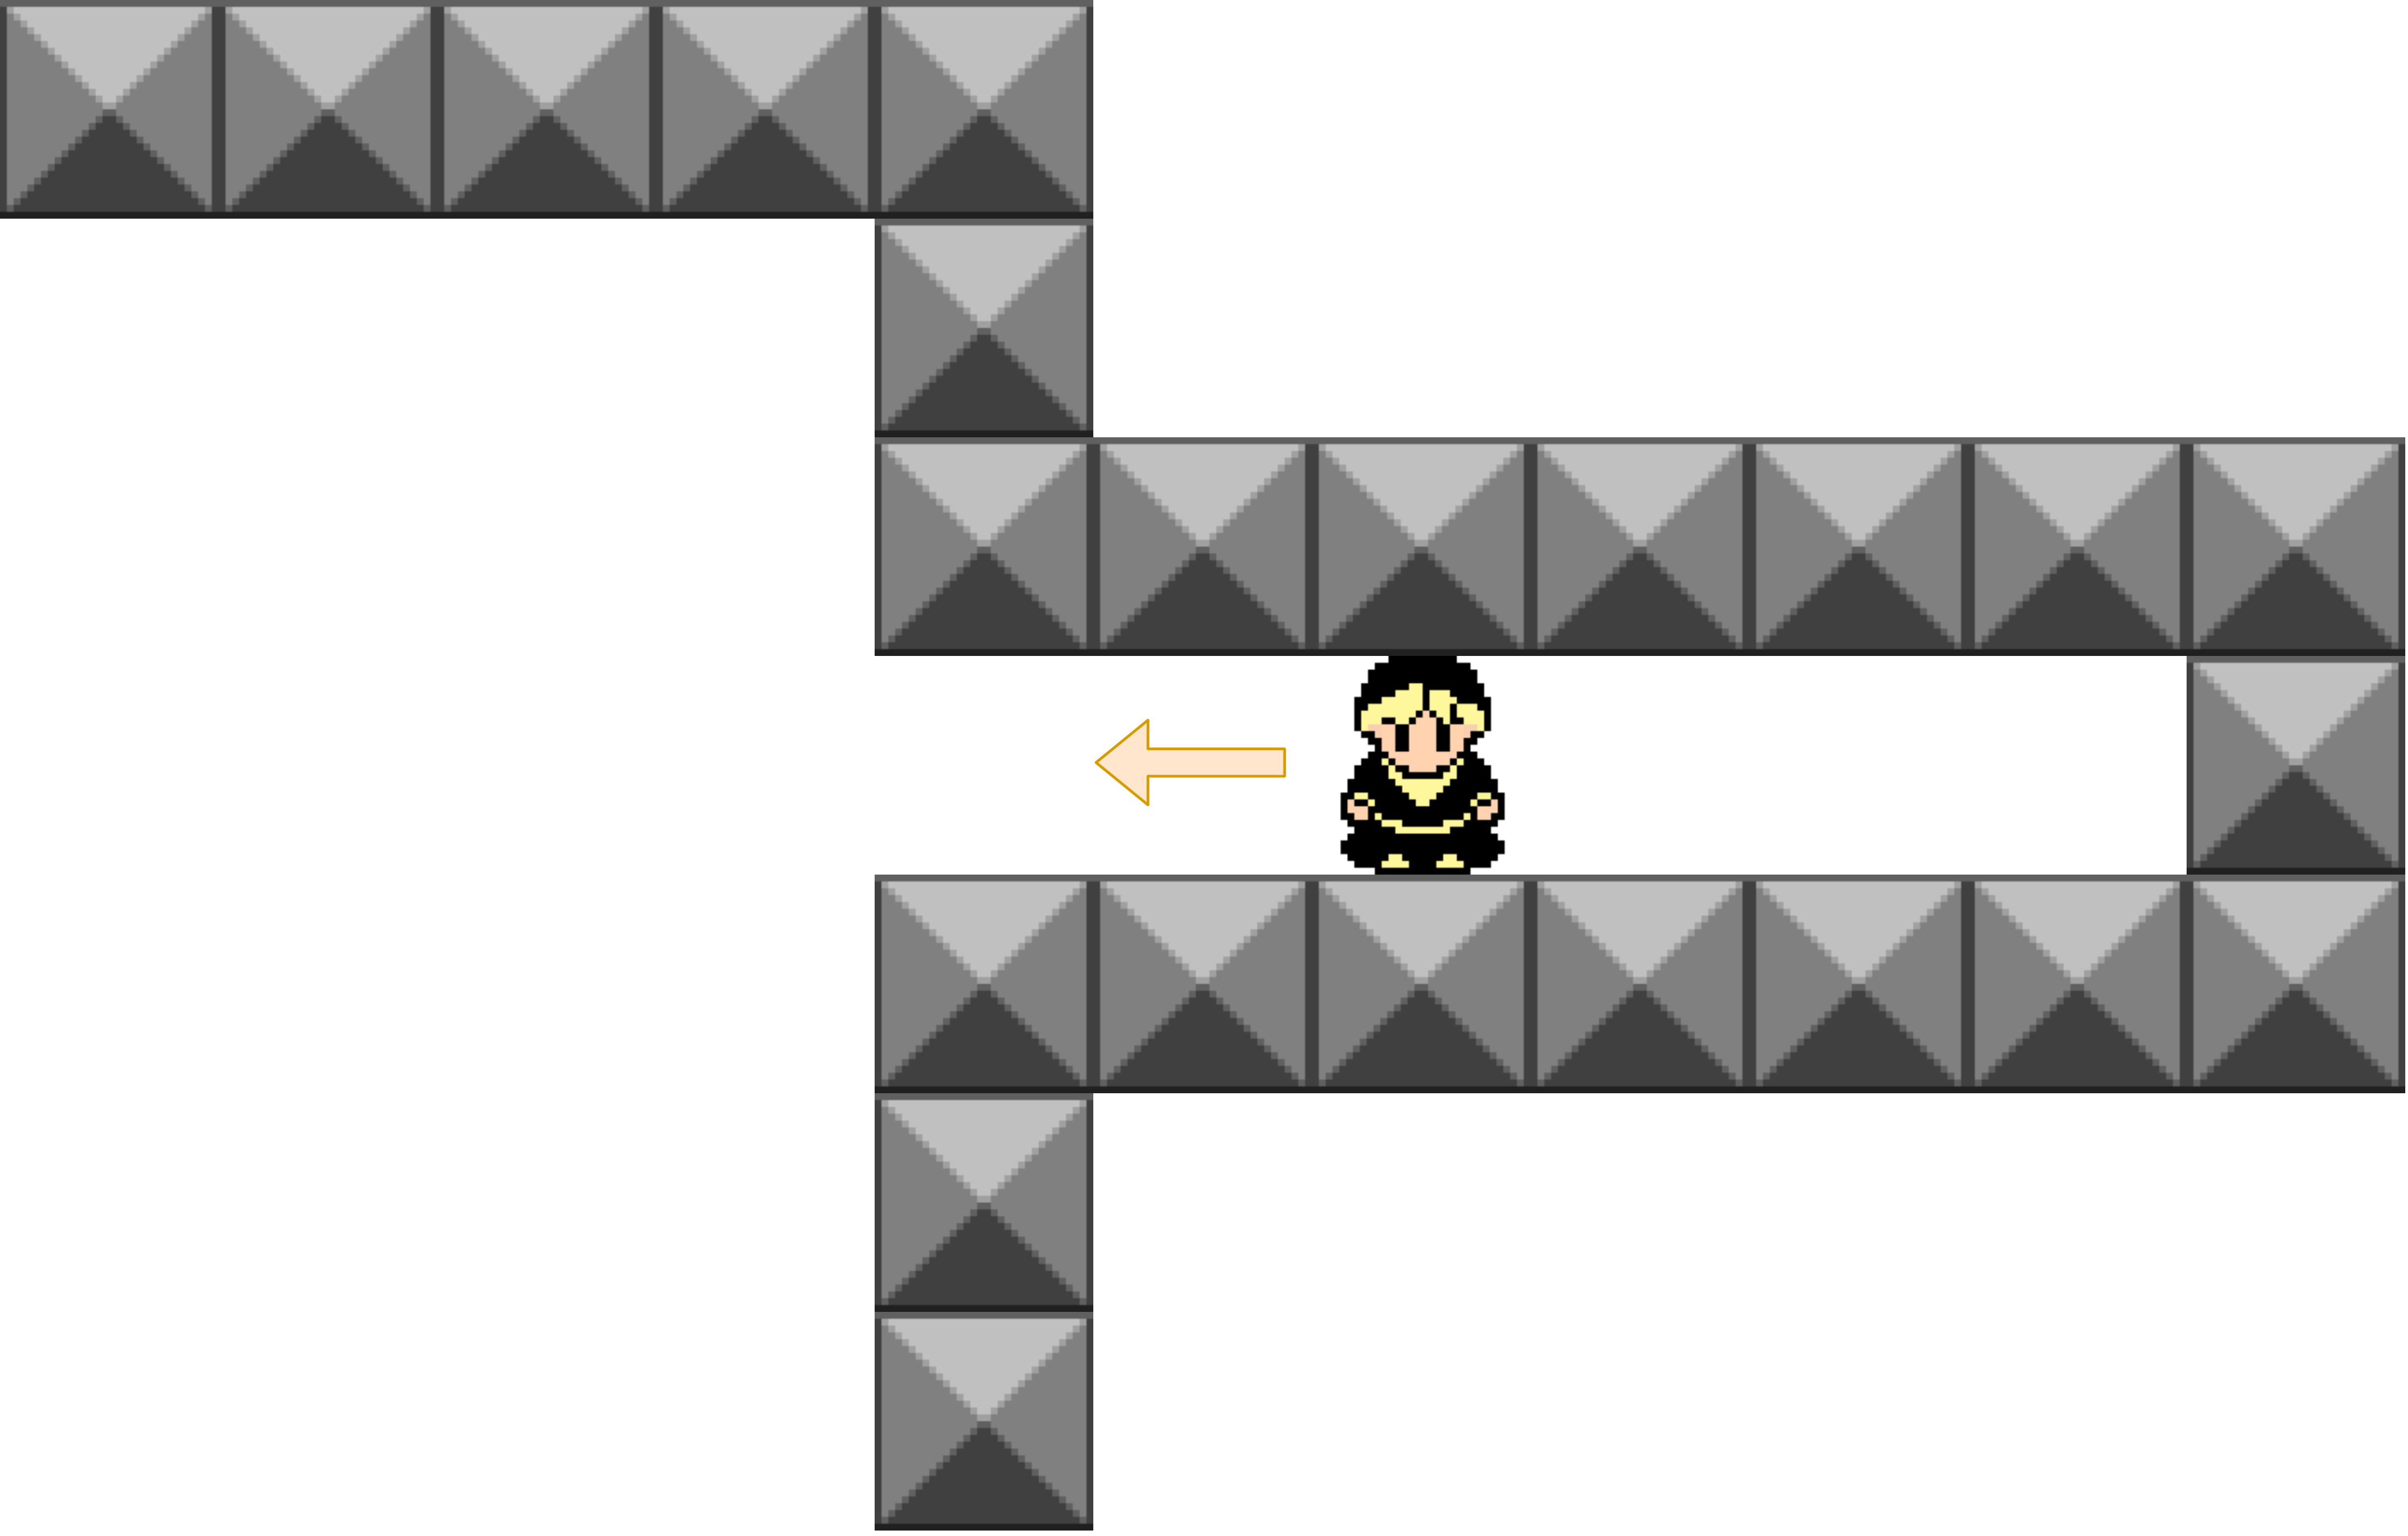
\includegraphics[width=1\textwidth]{example}
    \caption{Ejemplo de pasillo estrecho}
    \label{fig:ejemplo}
\end{figure}